\documentclass{article}

% Injects content from preamble.tex (mostly imports) here
%%%%% IMPORTS %%%%%
% \usepackage{fourier} % Cool font
\usepackage{graphicx} % Required for inserting images
\usepackage{hyperref} % Required for \href for hyperlinks
\usepackage{amsmath, amsthm, amsfonts} % amsthm is for theorems. amsfonts is for \mathbb (etc.)

% Define theorem and corollary environments
% Required args in {}.
% Optional arg in [] defines numbering.
\newtheorem{theorem}{Theorem}
\newtheorem{corollary}{Corollary}

\newcommand{\R}{\mathbb{R}}
% [2] means 2 arguments
% #1 means first argument and #2 means second argument
\newcommand{\cv}[2]{\begin{bmatrix}#1\\#2\end{bmatrix}}

\usepackage{listings} % For code listings

\usepackage[
backend=biber,
style=alphabetic,
sorting=ynt
]{biblatex} % Bibliography
\addbibresource{refs.bib}


%%%%%%%%%% IGNORE %%%%%%%%%%
\usepackage{xcolor}

\definecolor{codegreen}{rgb}{0,0.6,0}
\definecolor{codegray}{rgb}{0.5,0.5,0.5}
\definecolor{codepurple}{rgb}{0.58,0,0.82}
\definecolor{backcolour}{rgb}{0.95,0.95,0.92}

\lstdefinestyle{mystyle}{
    backgroundcolor=\color{backcolour},   
    commentstyle=\color{codegreen},
    keywordstyle=\color{magenta},
    numberstyle=\tiny\color{codegray},
    stringstyle=\color{codepurple},
    basicstyle=\ttfamily\footnotesize,
    breakatwhitespace=false,         
    breaklines=true,                 
    captionpos=b,                    
    keepspaces=true,                                     
    numbersep=5pt,                  
    showspaces=false,                
    showstringspaces=false,
    showtabs=false,                  
    tabsize=2
}

\lstset{style=mystyle}

\usepackage{tcolorbox} % Theorem boxes
\tcbuselibrary{theorems}
\newtcbtheorem[number within=subsection]{exercise}{Exercise}{colback=magenta!5, colframe=magenta!35!black,fonttitle=\bfseries}{th}
\newtcbtheorem[number within=subsection]{solution}{Solution}{colback=green!5, colframe=green!35!black,fonttitle=\bfseries}{th}

\usepackage{commath}
%%%%%%%%%% IGNORE %%%%%%%%%%


\title{\LaTeX{} Workshop Demo (complete)}
\author{Jesse Wei}
\date{March 26, 2024}

\begin{document}

\maketitle

\tableofcontents
\newpage

\section{Introduction}

This is our \LaTeX{} workshop's complete demo (template \href{https://www.overleaf.com/read/tmgncmqywbdj#3f2451}{here}). Here are the associated \href{https://docs.google.com/presentation/d/1zO6tLPnshC0WfSBvqL2mZKDLLprnuQr2t1IMmsjBdlM/edit?usp=sharing}{slides}. This demo is heavily inspired by \cite{latex_vid_1} and \cite{latex_vid_2}.

\section{Math formatting}

Let's write some expressions involving the number $e$.

\subsection{Math mode (inline)}

$e=2.71828$

\subsection{Math mode (display)}

$$e=2.71828$$

\subsection{Expressions}

% fraction
$$(1+\frac{1}{n})^n$$

% left right
$$\left(1+\frac{1}{n}\right)^n$$

% subscript
$$\lim_{n\to\infty}\left(1+\frac{1}{n}\right)^n$$

% sqrt and (optional) argument [n]
$$\lim_{n\to\infty}\frac{n}{\sqrt[n]{n!}}$$

% superscript, sum
$$\sum_{n=0}^{\infty}\frac{1}{n!}$$

% numbered equation with label
\begin{equation}
    \label{esum}
    \sum_{n=0}^{\infty}\frac{1}{n!}
\end{equation}

Since we labeled the above equation with \texttt{\textbackslash label\{esum\}}, we can refer to it with \texttt{\textbackslash ref}, like so: \ref{esum}.

%%%%%%%%%%%%%%%%%%
% Pause demo for 2 min to allow students to write their own.
% Or they can skip to exercise
%%%%%%%%%%%%%%%%%%

\subsection{Symbols}

Some lowercase symbols: $\alpha, \beta, \gamma, \sigma, \rho, \pi$

Uppercase symbols: $\Gamma, \Sigma, \Pi$

Symbols sometimes look different in inline and display mode even when the code is the same. For example,

$\sum_{i=0}^n$

$$\sum_{i=0}^n$$

$\prod_i$

$$\prod_i$$

\subsection{How to find symbol}

% Note: do not use " " (double quotation marks)
% Instead, use `` " (two grave symbols, then a quotation mark)
Is there a symbol that you don't know how to write in \LaTeX? You could try \href{https://detexify.kirelabs.org/classify.html}{Detexify} \footnote{Link made possible by \textbackslash usepackage\{hyperref\} in the preamble}, but I don't find it that great. Instead, I recommend googling (e.g., ``How to type alpha in LaTeX").

\subsubsection{Exercise}

\begin{exercise}{Expressions and symbols}{}
    Transcribe the following. If you don't know how to write a symbol in \LaTeX, search up how to write it. Once you're done, you can compare with \texttt{solutions/expressions.tex}.

    \begin{enumerate}
    \item $\sum_{n=1}^{2024}\frac{1}{n}$
    \item $x=\frac{-b \pm \sqrt{b^2-4ac}}{2a}$
    \item $\od[2]{f}{x}$ % Nitpick: Use \od from package commath for non-italicized d. Up to you whether or not little details like this matter, but good to know stuff like this exists
    
    \item $\int_a^b f(x) \dif x$  % Same here, \dif
    
    \item $
        \begin{bmatrix}
            1 & 0 & 0\\
            0 & 1 & 0\\
            0 & 0 & 1\\
        \end{bmatrix}
        $
\end{enumerate}
\end{exercise}

\begin{solution}{}{}
    \begin{enumerate}
        \item 
        \item 
        \item 
        \item 
    \end{enumerate}
\end{solution}

\section{Text formatting}

\subsection{Text}

\textbf{Bold}, \textit{Italicize}, \underline{underline}, footnote\footnote{This is a footnote}

\subsection{Lists}

\begin{enumerate}
    \item 1
    \item 2
    \item 3
\end{enumerate}

\begin{itemize}
    \item 4
    \item 5
    \item 6
\end{itemize}

If you forget the source code for these, you can click $\cdots >$ Bullet list or Numbered List in the Overleaf UI at the top.

\subsection{Figures}

Click $\cdots >$ Insert Figure $>$ From project files in the Overleaf UI to insert \texttt{img/latex.png}.

\begin{figure}[h]
    \centering
    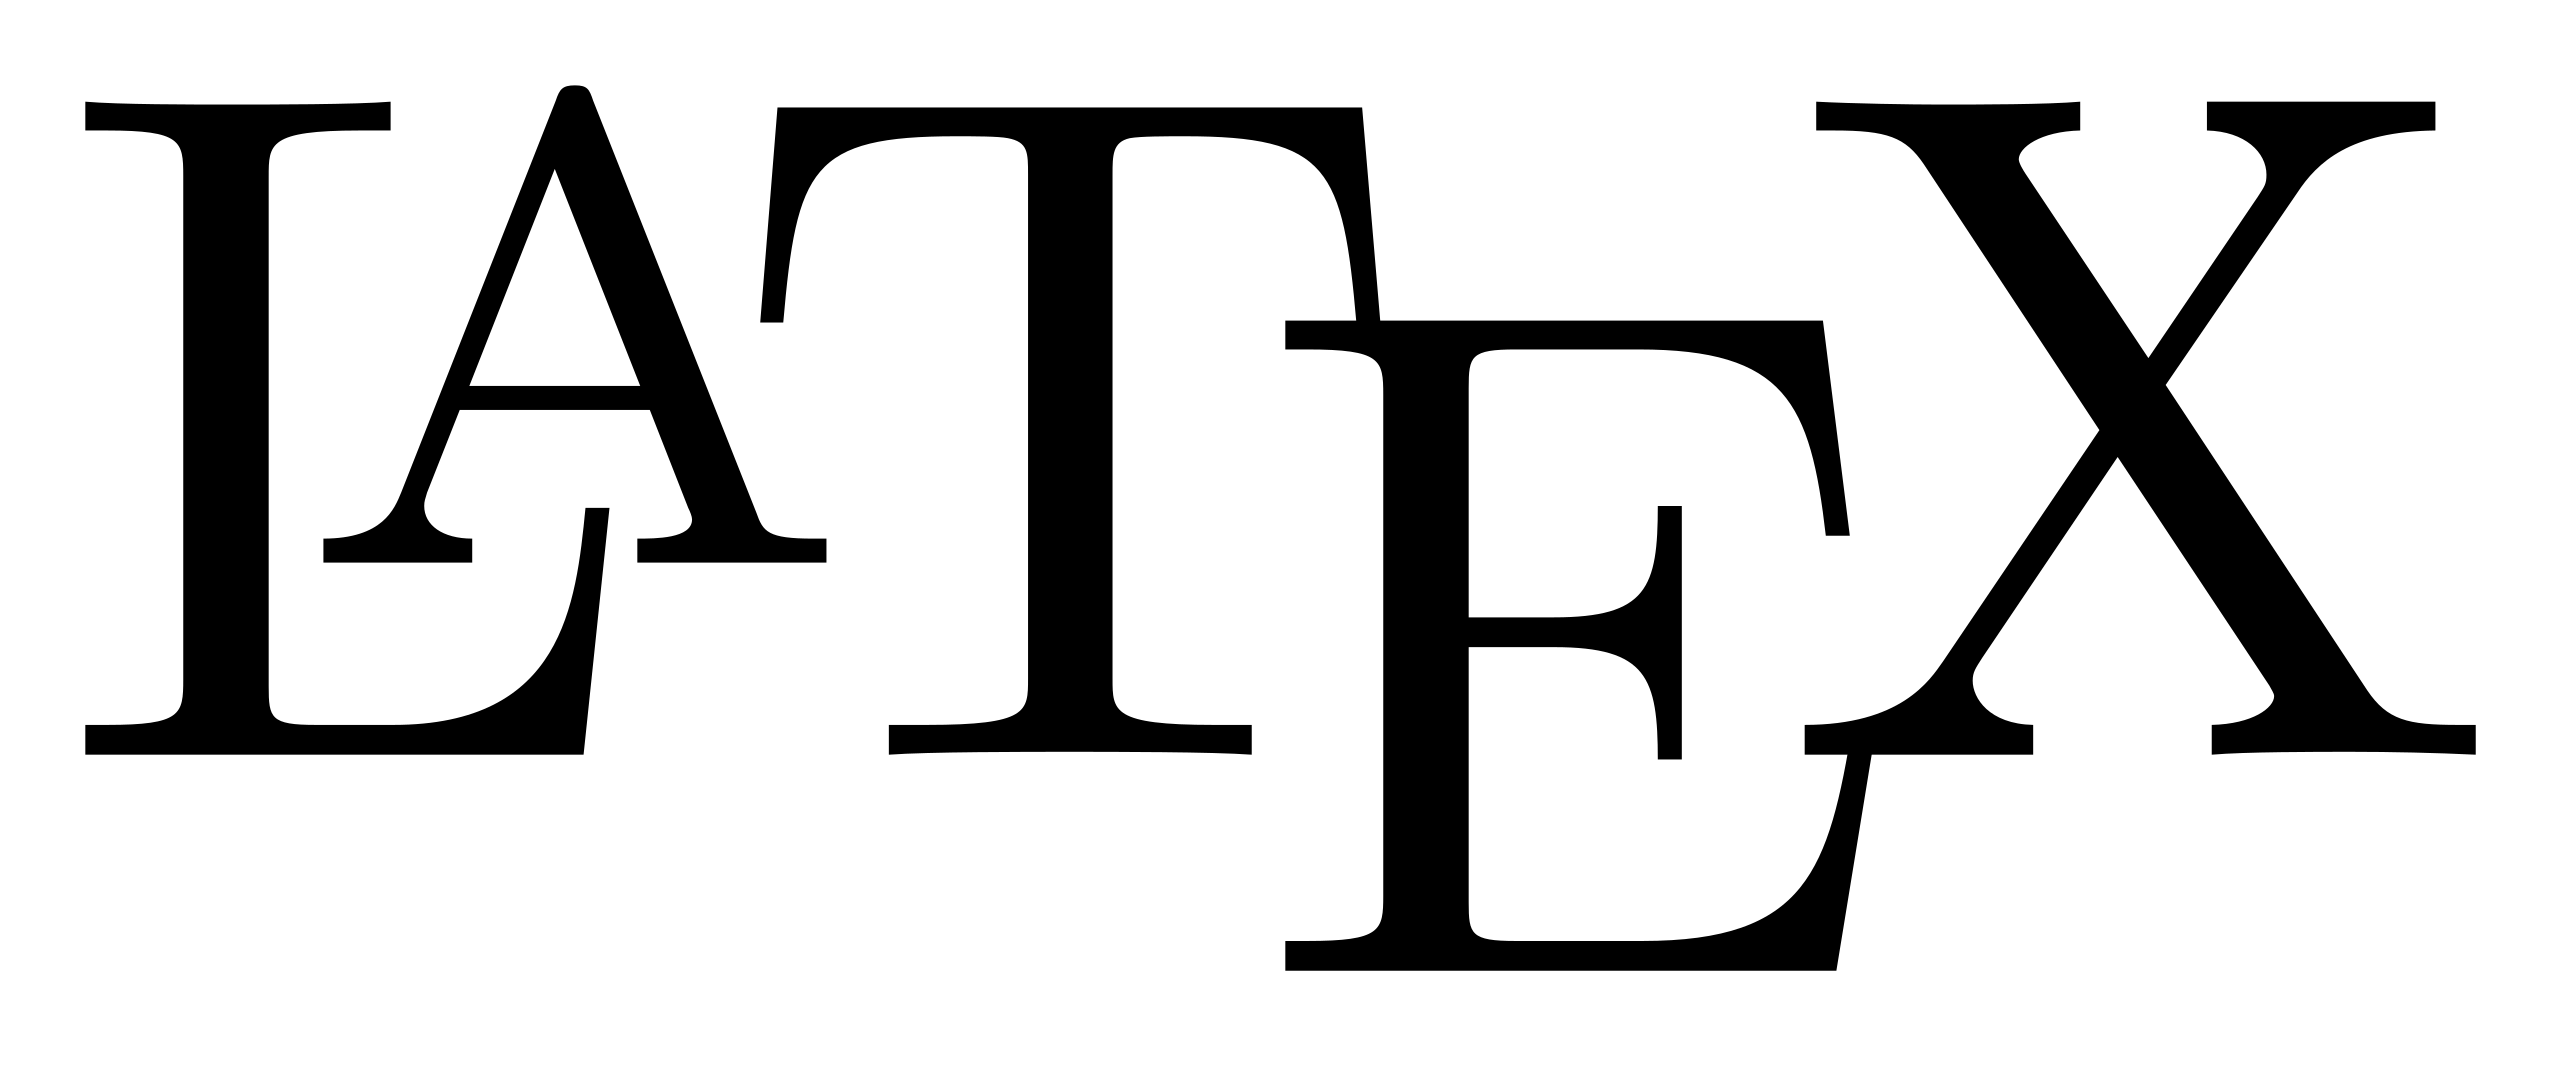
\includegraphics[width=0.6\linewidth]{img/latex.png}
    \caption{\LaTeX{} logo}
    \label{latex_logo}
\end{figure}

If we label it with \texttt{\textbackslash label}, we can refer to it using \texttt{\textbackslash ref}, like so \ref{latex_logo}.

The figure will probably go somewhere unexpected (i.e., some location that isn't where you wrote \textbackslash begin\{figure\} because \LaTeX{} decides where it goes. For example, if there isn't enough space on the current page, then the figure will be placed on the next page. Try removing [h] from the above source code, and see where the figure goes.

We can sometimes resolve this with \texttt{\textbackslash begin\{figure\}[h]}. If that doesn't work, you may have to use \texttt{\textbackslash pagebreak} or other means.

\subsection{Tables}

Click Insert table at the top of the UI. Similar to figures, tables also may not go where you want without [h] or other means.

\begin{table}[h]
    \centering
    \begin{tabular}{ccc}
        1 & 2 & 3\\
        4 & 5 & 6\\
        7 & 8 & 9\\
    \end{tabular}
    \caption{No lines}
\end{table}

You can add lines:

\begin{table}[h]
    \centering
    \begin{tabular}{|c|c|c|}
        \hline
        1 & 2 & 3\\
        \hline
        4 & 5 & 6\\
        \hline
        7 & 8 & 9\\
        \hline
    \end{tabular}
    \caption{With lines}
\end{table}

\subsection{Comments}

Write a comment for your source code using \%.

For example, there's an unrendered comment here $\rightarrow$ % this is a comment and isn't rendered

\subsection{Escape characters}

However, if \% denotes a comment, how do we write \% in text? Use \textbackslash to escape the reserved character. And note that \textbackslash is also reserved, so to write \textbackslash, this source code uses \texttt{\textbackslash textbackslash}.

\subsubsection{Exercise}

\begin{exercise}{Escape characters}{}
    Transcribe the following. Once you're done, you can compare with \texttt{solutions/escape.tex}.

    \begin{enumerate}
    \item \$, \&, and $\sim$
    \item $x=\{1,2,3\}$
    \item $\text{rain} \implies \text{bring umbrella} \implies \text{use umbrella}$
\end{enumerate}

    3 should be done in math mode (for the sake of example), and use \texttt{\textbackslash text} to escape math mode.
    
\end{exercise}

\begin{solution}{}{}
    \begin{enumerate}
        \item 
        \item 
        \item
    \end{enumerate}
\end{solution}

\subsection{Code}

For inline code, it's good practice to use \texttt{\textbackslash texttt}, which is a monospace code-looking font. For example, \texttt{print("hello world")}.

For longer code listings, use the \texttt{listings} package. For example,

\begin{figure}[h]
    \centering
    \begin{lstlisting}[language=Python]
    def bogosort(l: list[int]):
        """Bogosorts list of integers"""
        while not sorted(l) == l:
            shuffle(l)
    \end{lstlisting} 
\end{figure}

See \cite{overleaf_code} for more information.

\section{Define our own formatting}

\subsection{Environments}

%%%%%%%%%%%%
% Add [section] and [theorem] to preamble after
%%%%%%%%%%%%

When we use \texttt{\textbackslash begin} and \texttt{\textbackslash end}, we enter environments. We can actually define our own environments. For example, see the \texttt{\textbackslash newtheorem} definitions in \texttt{preamble.tex}.

\begin{theorem}
    There are no solutions to $a^n+b^n=c^n$ for positive integers $n > 2$.
\end{theorem}

\begin{proof}
    Left as an exercise to the reader.
\end{proof}

\begin{theorem}
    P=NP
\end{theorem}

\begin{proof}
    Left as an exercise to the reader.
\end{proof}

\begin{corollary}
    All of cryptography\footnote{except OTP} is broken.
\end{corollary}

\subsection{Macros}

Macros help us automate repetitive tasks.

For example, we normally write $\mathbb{R}$ with \texttt{\textbackslash mathbb\{R\}}. However, this is tedious to write every time. So, we can define a new command as a shortcut. For example, since we have \texttt{\textbackslash newcommand\{\textbackslash R\}\{\textbackslash mathbb\{R\}\}} in the preamble, we can simply write \texttt{\textbackslash R} to display $\R$.

As another example, suppose we want to implement a macro for column vectors. We can write a column vector using \texttt{bmatrix} (even inline). For example, $\begin{bmatrix}0\\1\end{bmatrix}$. However, this is a lot to type. So, check out the macro for \texttt{\textbackslash cv} in the preamble. Now, \texttt{\textbackslash cv\{0\}\{1\}} outputs $\cv{0}{1}$.

\section{Bibliography}

We can add a bibliography using the package \texttt{biblatex} and a \texttt{.bib} file.

See the \texttt{biblatex} import in \texttt{preamble.tex}. Also see \texttt{refs.bib}. You can cite a source using \texttt{\textbackslash cite}, like so \cite{latex_vid_1} \cite{latex_vid_2}. Then, use \texttt{\textbackslash printbibliography} to place the bibliography.

Note that if a source from the \texttt{.bib} file is not cited, it will not appear in the document.

See \cite{overleaf_bibliography} for more information.

\newpage
\printbibliography

\end{document}
